\begin{center}
    \resizebox{\linewidth}{!}{
        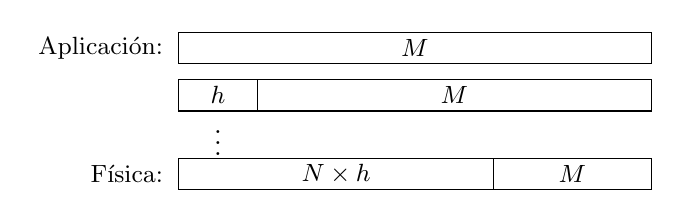
\begin{tikzpicture}
            \draw (-1, -0.2) node[text width=1.6cm, align=flush right]{\small Aplicación:};
            \draw (0,0)  rectangle node{\small $M$} +(6,-0.4);
            \draw (0,-0.6) rectangle node{\small $h$} +(1,-0.4);
            \draw (1,-0.6) rectangle node{\small $M$} +(5,-0.4);
            \draw (0.5, -1.3) node{$\vdots$};
            \draw (-1, -1.8) node[text width=1.6cm, align=flush right]{\small Física:};
            \draw (0, -1.6) rectangle node {\small $N \times h$} +(4,-0.4);
            \draw (4, -1.6) rectangle node {\small $M$} +(2,-0.4);
        \end{tikzpicture}
    }
\end{center}